\documentclass{article}

% Language setting
% Replace `english' with e.g. `spanish' to change the document language
\usepackage[english]{babel}
\usepackage{booktabs} 

% Set page size and margins
% Replace `letterpaper' with `a4paper' for UK/EU standard size
\usepackage[letterpaper,top=2cm,bottom=2cm,left=3cm,right=3cm,marginparwidth=1.75cm]{geometry}

% Useful packages
\usepackage{amsmath, amssymb, amsthm, mathtools, bm, lipsum}
\usepackage{graphicx}
\usepackage{geometry}

\usepackage[colorlinks=true, allcolors=blue]{hyperref}

\title{The mechanism of social plasticity determines when sociality helps or hinders adaptation}
\author{Andrea}

\begin{document}
\maketitle

\begin{abstract}
Phenotypic plasticity is often expected to help populations cope with environmental change. A subclass of plasticity is social plasticity where individuals could influence each other through social interactions and create feedback loops, and species may use different social rules. These properties make social plasticity different from other classes of plasticity whose evolutionary dynamics has been studied extensively. To study the evolutionary consequences of social plasticity, we use individual-based modeling with explicit genetic architecture to explore three social strategies: copying the group average, copying the fittest group member, and copying the most extreme group member. Under stabilizing selection, these mechanisms produced distinct genotype–phenotype relationships. Copy-the-average and copy-the-best reduced phenotypic variance, whereas copy-the-extreme produced non-monotonic changes in variance and could generate bimodal phenotypic distributions from approximately unimodal genetic variation. Across mechanisms, stronger social influence tended to maintain higher genetic variation, suggesting that social plasticity can weaken the relationship between genotype and expressed phenotype. After an environmental shift, only copy-the-best generated an immediate adaptive phenotypic response by allowing individuals to express phenotypes closer to the new optimum before substantial genetic change occurred. However, this short-term plastic benefit came with slower long-term genetic adaptation, a pattern also observed under copy-the-average and copy-the-extreme when social influence was strong or group size was large. In periodically fluctuating environments, the fitness consequences of sociality depended on the interaction rule, shift magnitude, and fluctuation frequency. Copy-the-best provided the broadest fitness advantage, while copy-the-average and copy-the-extreme were beneficial only under more limited environmental conditions and became costly when shifts were large or social influence was strong. These results show that social plasticity is not inherently adaptive. Instead, whether sociality helps or hinders adaptation depends on what individuals copy, how strongly they copy, and how rapidly the environment changes.

\end{abstract}

\section{Introduction}

% intro to IGE

% how is IGE manifested through social learning

\section{Model}
Our model is built upon two different models: the IGE model proposed by \cite{Moore1997} and an evolutionary quantitative trait framework developed by \cite{Hayward2022}. Individuals' phenotype is affected by a highly polygenic genotype and social partners. Genotype of the trait under selection follows the standard additive model with a highly polygenic genetic basis \cite{Hayward2022, Falconer1996} and that one individual's genotype is given by 
\begin{equation}
a = \sum_k x_{k},
\label{g_def}
\end{equation}
where $x_k$ is the effect size of $k^{th}$ mutation of the individual. The genetics of the trait under selection is assumed to follow the infinitesimal model \cite{Fisher1918}. $x$ is drawn from a Rayleigh distribution with $\sigma=\frac{1}{\sqrt{2}}$ with equal chance of being negative or positive. The mutation rate per generation is $U=0.03$ \cite{Hayward2022}.

The social interaction model is inspired by \cite{Moore1997} and we extend the model to include multiple social partners as well as nonlinear interactions. During each generation, individuals are partitioned to a group of $n$ individuals, and they are each other's social partners. One individual's phenotype is defined as 
\begin{equation}
\label{eq:z_def}
z = (1-\psi)g+\psi g_{social} +e
\end{equation}
where $\psi$ is the interaction coefficient, $g_{social}$ is the indirect genetic effect from the individual's social partners, and $e$ is the general environmental effect. $\psi$ stays as a constant for the entire simulation, and $g_{social}$ is calculated differently based on the different interaction model defined in Section \ref{sec:interaction_models} and Fig. \ref{fig:model_fig}B. 

It is worth noting that $\psi$ is defined slightly different here than in \cite{Moore1997}. As the interaction coefficient, $\psi$ represents how much does one's phenotype depend on social partners. In the original model, the contribution of one's genotype to the phenotype is not explicitly defined. Rather, the proportion of phenotype that's determined by own genotype depends on the absolute value of its social partner's genotype. As a result of not being translational invariant, we redefined $\psi$ to be the proportion of which one's phenotype is composed by the effect from social partners. Thus, $\psi\geq0$ is required in our study. See Appendix X for more discussion (NOTE: The comparison between our model and their model will be put in appendix).

Our model assumes a standard diploid Wright-Fisher population with a constant size $N$ and non-overlapping generations. The simulations are done in SLiM \cite{Haller2023}. In each generation, the population is randomly partitioned into group of size $n$ to calculate each individual's phenotype. Notably, grouping only influence phenotype expression; mating and reproduction events treats the population as panmictic. (NOTE: a table of symbols and annotations used, insert here or appendix).


% \begin{table}[ht]
% \centering
% \caption{Default simulation parameters}
% \label{tab:default_parameters}
% \begin{tabular}{llll}
% \hline
% Symbol  & Default value & Description \\
% \hline
% $N$  & 10000 & Number of individuals per generation \\
% $n$  & - & Group size \\
% $\psi$  & - & Social interaction coefficient \\
% $L$  & - & Number of loci \\
% $\mu$  & $1\times10^{-5}$ & Mutation rate \\
% $\sigma_m$ & Mutational effect SD & 0.1 & Standard deviation of mutational effects \\
% $\omega^2$ & Selection strength & 10 & Width of Gaussian stabilizing selection \\
% $\theta$ & Phenotypic optimum & 0 & Environmental optimum before shift \\
% $\Delta\theta$ & Optimum shift size & 20 & Magnitude of environmental shift \\
% $T$ & Total generations & 20000 & Length of simulation \\
% \hline
% \end{tabular}
% \end{table}

\begin{figure}
    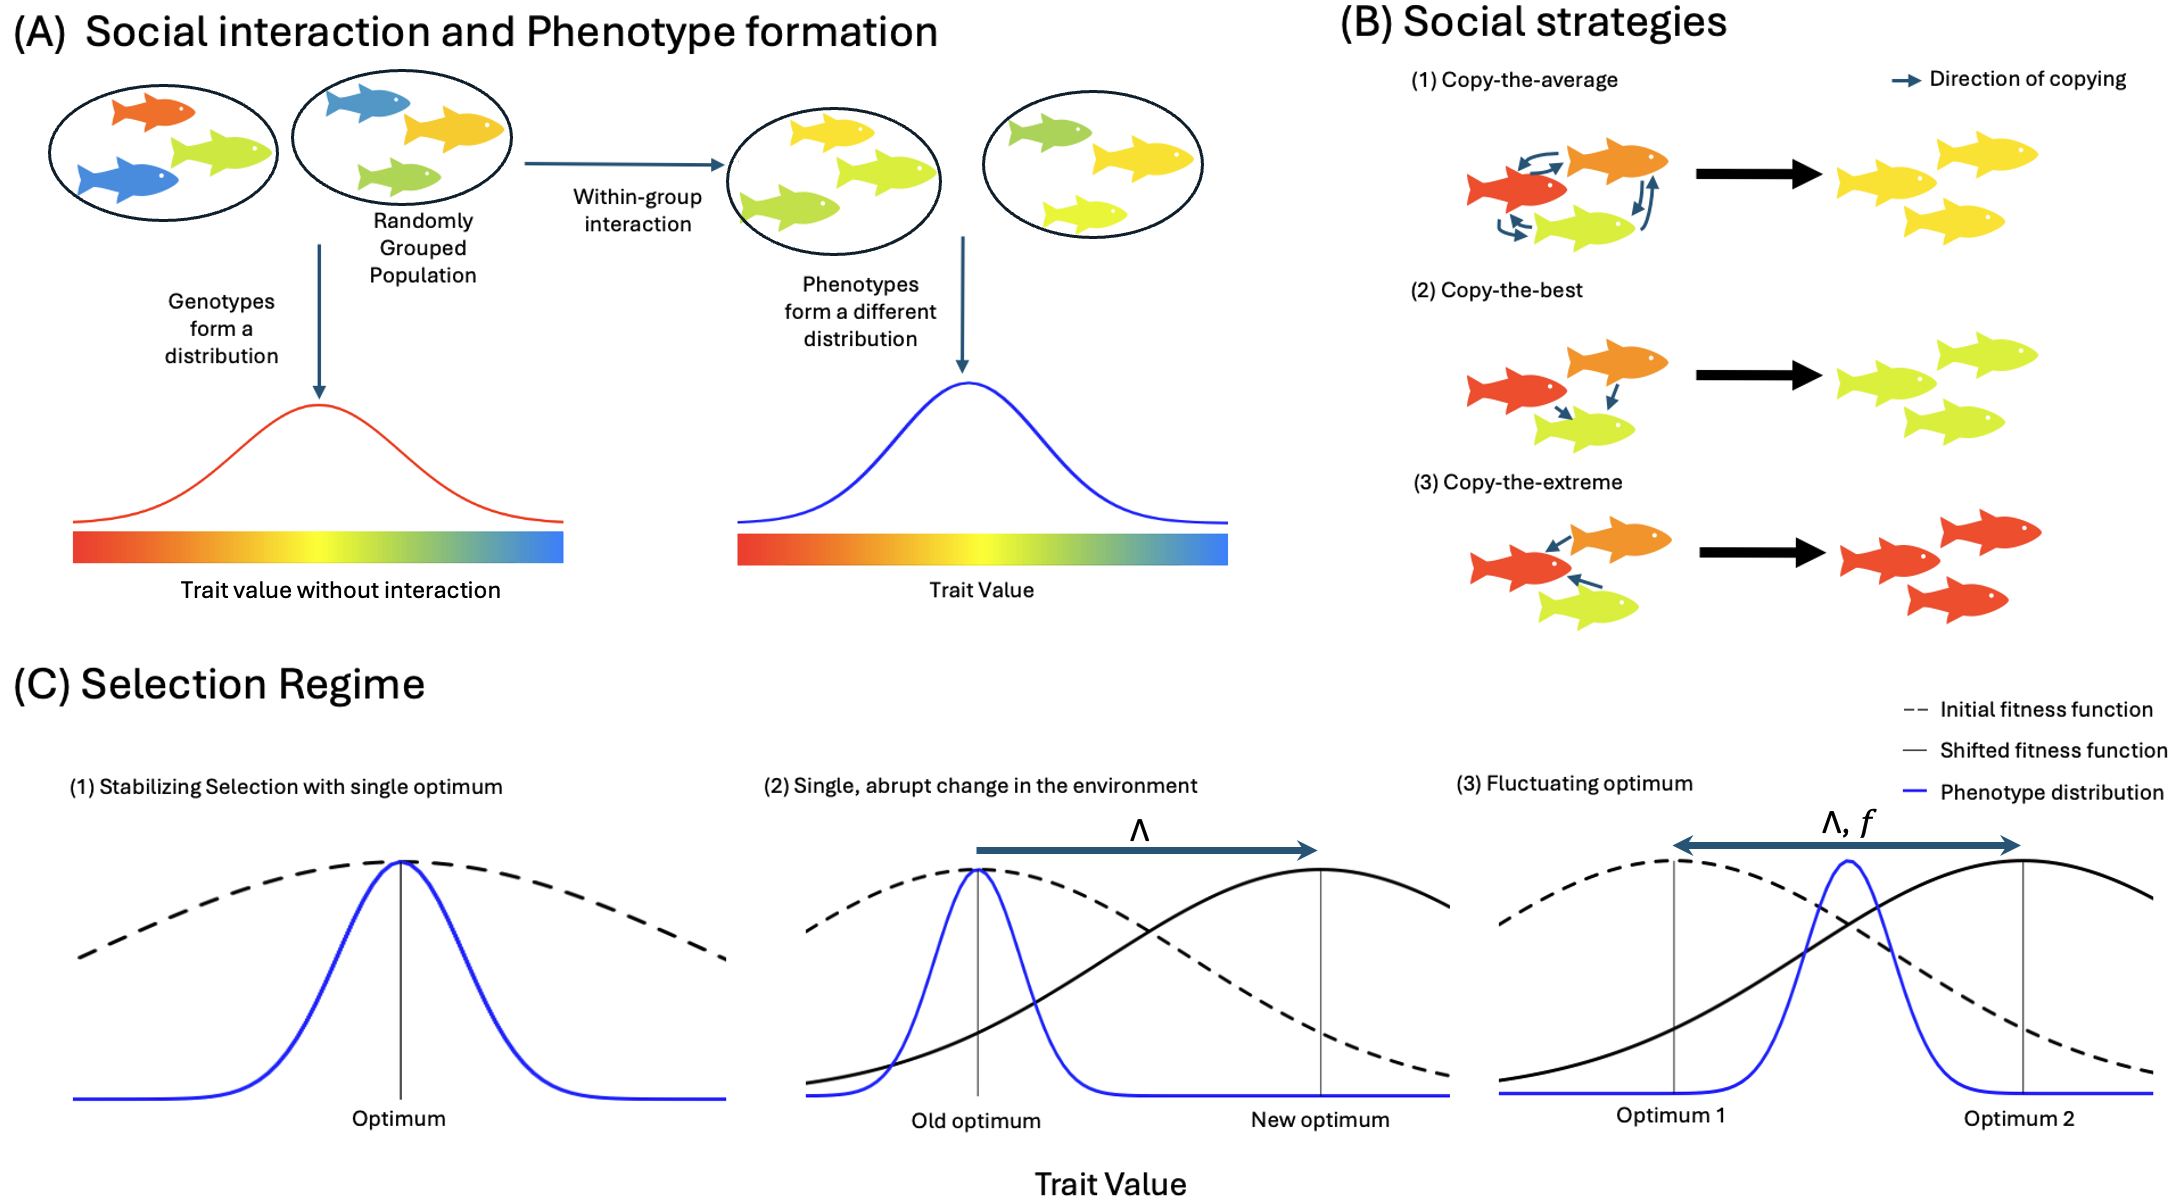
\includegraphics[width=\linewidth]{fig/model_fig.png}
    \caption{\textbf{Overview of the model structure.} (A) Within each generation, individuals are randomly partitioned into groups. Genotypes form a population-level distribution, and within-group interactions determine phenotype expression, generating a potentially different phenotype distribution. (B) Social interaction strategies modeled included copy-the-average, copy-the-best, and copy-the-extreme, which determine how do one's phenotype affected by group members. See \ref{sec:interaction_models}. (C) Selection regimes examined: (1) long-term stabilizing selection under a single fitness optimum, (2) a single abrupt shift in the optimum with magnitude $\Lambda$ after the stabilizing selection, and (3) a fluctuating optimum that alternates between two trait values at frequency $f$. Dashed and solid curves indicate the initial and shifted fitness functions, respectively; blue curves denote phenotype distributions.}
    \label{fig:model_fig}
\end{figure}

\subsection{Social Interaction Models}
\label{sec:interaction_models}
After individuals are assigned to a group of size $n$, the phenotype of each individual is calculated as Eq \ref{eq:z_def}. In this study, we consider three different strategies that determines the value of $g_{social}$ for an individual's phenotype: copy the average, copy the best, and copy the extreme. 

\paragraph{Copy-the-Average} As we adopt the model in \cite{Moore1997}, the third paper in the same series extends the group size from 2 to $n$ individuals \cite{McGlothlin2010}. The assumption was that the focal individual is influenced by the mean phenotype of all its social partners. This formulation corresponds to a form of frequency-dependent social influence in which individuals adjust their phenotype toward the tendency of the group. Conceptually, this is closely related to conformist transmission in social learning theory, where individuals disproportionately adopt the most common behavior in the population in an evolutionary setting \cite{Boyd1985}. In binary decision context, conformity is often represented by "copy-the-majority", leading the group to one of the two choices. However, our trait space is continuous, meaning that there is no discrete majority category; instead, we model conformity as adjustment toward the group mean, which in term approaches the population mean. With a symmetric trait distribution, the mean is also the most frequent phenotype, so copy-the-average provides a continuous analogue of majority-based social learning.

(NOTE: I'll add a discussion of why this strategy makes sense and include biological examples) (citations: \cite{Laland2004})


Specifically, the single-trait model from \cite{Moore1997} is extended to allow group of $n$ individuals; for the $i^{th}$ individual in the group, its phenotype is: 

\begin{equation}
z_i = (1-\psi)g_i + e_i + \psi \frac{1}{n-1} \sum_{j \ne i} z_j 
\label{eq:system}
\end{equation}
where $g_i$ denotes the direct genetic effect, $e_i$ an environmental effect, and $\psi$ the social interaction coefficient (Fig \ref{fig:model_fig}B1). Solving this linear system (Appendix X) yields

\begin{equation}
z_i
=
\frac{n-1}{n-1+\psi}\big((1-\psi)g_i + e_i\big)
+
\frac{\psi}{n-1+\psi}
\left(
\sum_{k=1}^n g_k
+
\frac{\sum_{k=1}^n e_k}{1-\psi}
\right).
\label{eq:ave_eq}
\end{equation}
The solution exists for $\psi\ne 1$; at $\psi =1$ the system becomes singular. Given our definition of $\psi$ as a proportion coefficient, we keep $\psi\in [0,1)$ throughout the rest of the study.


\paragraph{Copy-the-Best}
In our model, we aggregate the cumulative effect of social interactions across an individual's lifetime into a single value in phenotype and fitness outcome. However, many biological interactions involves repeated encounters over the lifetime, such as (examples like best-of-n mate choice strategy and choosing nest location). These repeated interactions may allow individuals to assess the success of their group mates' phenotype and adjust their behavior accordingly, for example by copying the most successful neighbor. To capture this dynamics, we adopt a simple yet biologically reasonable model in which individuals assess the fitness of its social partners' genotype and copy the genotype of the individual with the highest fitness \cite{Laland2004} (Fig \ref{fig:model_fig}B2). Specifically, the model for copy-the-best strategy for a group of size $n$ is 
\begin{equation}
    z_i = (1-\psi)g_i+e_i+ \psi g_{j^*} \text{ where }j^*=\arg\max_{j\in n}(W(g_j)).
\end{equation}
Note that individuals are allowed to copy themselves, i.e. $z_{j^*}=g_{j*}$, if they have the best genotype.

\paragraph{Copy-the-Extreme}
Frequency-dependent strategies usually comes with the form of copy-the-majority, but in rare cases, the minority of the group has more influence on others \cite{Laland2004}. A recent study has shown that a frequency as low as 20\% of an alternative genotype in a fire ant colony can convert the colony from monogyne to polygyne \cite{Zeng2025}. To implement this strategy in a model with continuous trait values, we define "copy-the-extreme" as copying the group member whose genotype deviates most strongly from the group mean. This formulation is motivated by the assumption that genotypes are approximately normally distributed in the population as well as within group \cite{Lande1976}. Under such a distribution, individuals that are far from the mean are also relatively rare. Thus, copying the most extreme genotype can capture the tendency of preferring an uncommon phenotype (Fig \ref{fig:model_fig}B3). The model is defined as 
\begin{equation}
    z_i = (1-\psi)g_i+e_i+ \psi g_{j^*} \text{ where }j^*=\arg\max_{j\in n}(|g_j-\bar{g}|).
\end{equation}


\subsection{Evolutionary Scenarios}

The population is simulated under three different selection regimes. All of them are implemented by changing the mean of the fitness function. Specifically, the fitness function, $W$, is assumed to be Gaussian with a mean of $\mu$ and a standard deviation of $\sigma$, where $\mu$ is the fitness optimum for the population. The fitness function assumes that fitness declines with the distance between phenotype and the fitness optimum. We adopted an evolutionary framework from \cite{Hayward2022}. In their work, the population is under long-term stabilizing selection until a abrupt change in the environment represented by a change in the fitness optimum; they investigate the dynamics of the allele frequency of a highly polygenic trait whose genotype is directly under selection. Inspired by their work, we look at three different evolutionary scenarios: long-term stabilizing selection, directional selection from the change in fitness optimum, and periodically fluctuating environment. 

\paragraph{Stabilizing Selection} The environment is assumed to be stable and has a single optimum for the trait (Fig \ref{fig:model_fig}C1). The population is placed under this fitness function with $\sigma=\sqrt{2N}$ for $10N$ generations for the population to reach mutation-selection-drift balance with $N$ being the population size \cite{Hayward2022}. 

\paragraph{Shift in Fitness Optimum} After the population is at the mutation-selection-drift balance, the fitness optimum shifts at $t_s=10N$ generation with a magnitude of $\Lambda$ (Fig \ref{fig:model_fig}C2). $\Lambda$ is kept constant across models and simulations as a parameter of interest. We are interested in how the trajectory of population adaptation to the new optimum changes with different social strategies and interaction coefficients.

\paragraph{Periodically Fluctuating Environment} As an extension to the single optimum shift, the population is instead placed under a fitness function that shift between two optimum values, $-\frac{\Lambda}{2}$ and $\frac{\Lambda}{2}$, with a frequency of $f$ generations (Fig \ref{fig:model_fig}C3) (NOTE: I'm not sure if we should going through stabilizing selection first or just do fluctuating environment which is what I'm doing right now)

\section{Result}

\subsection{Stabilizing Selection}
\begin{figure}
    \centering
    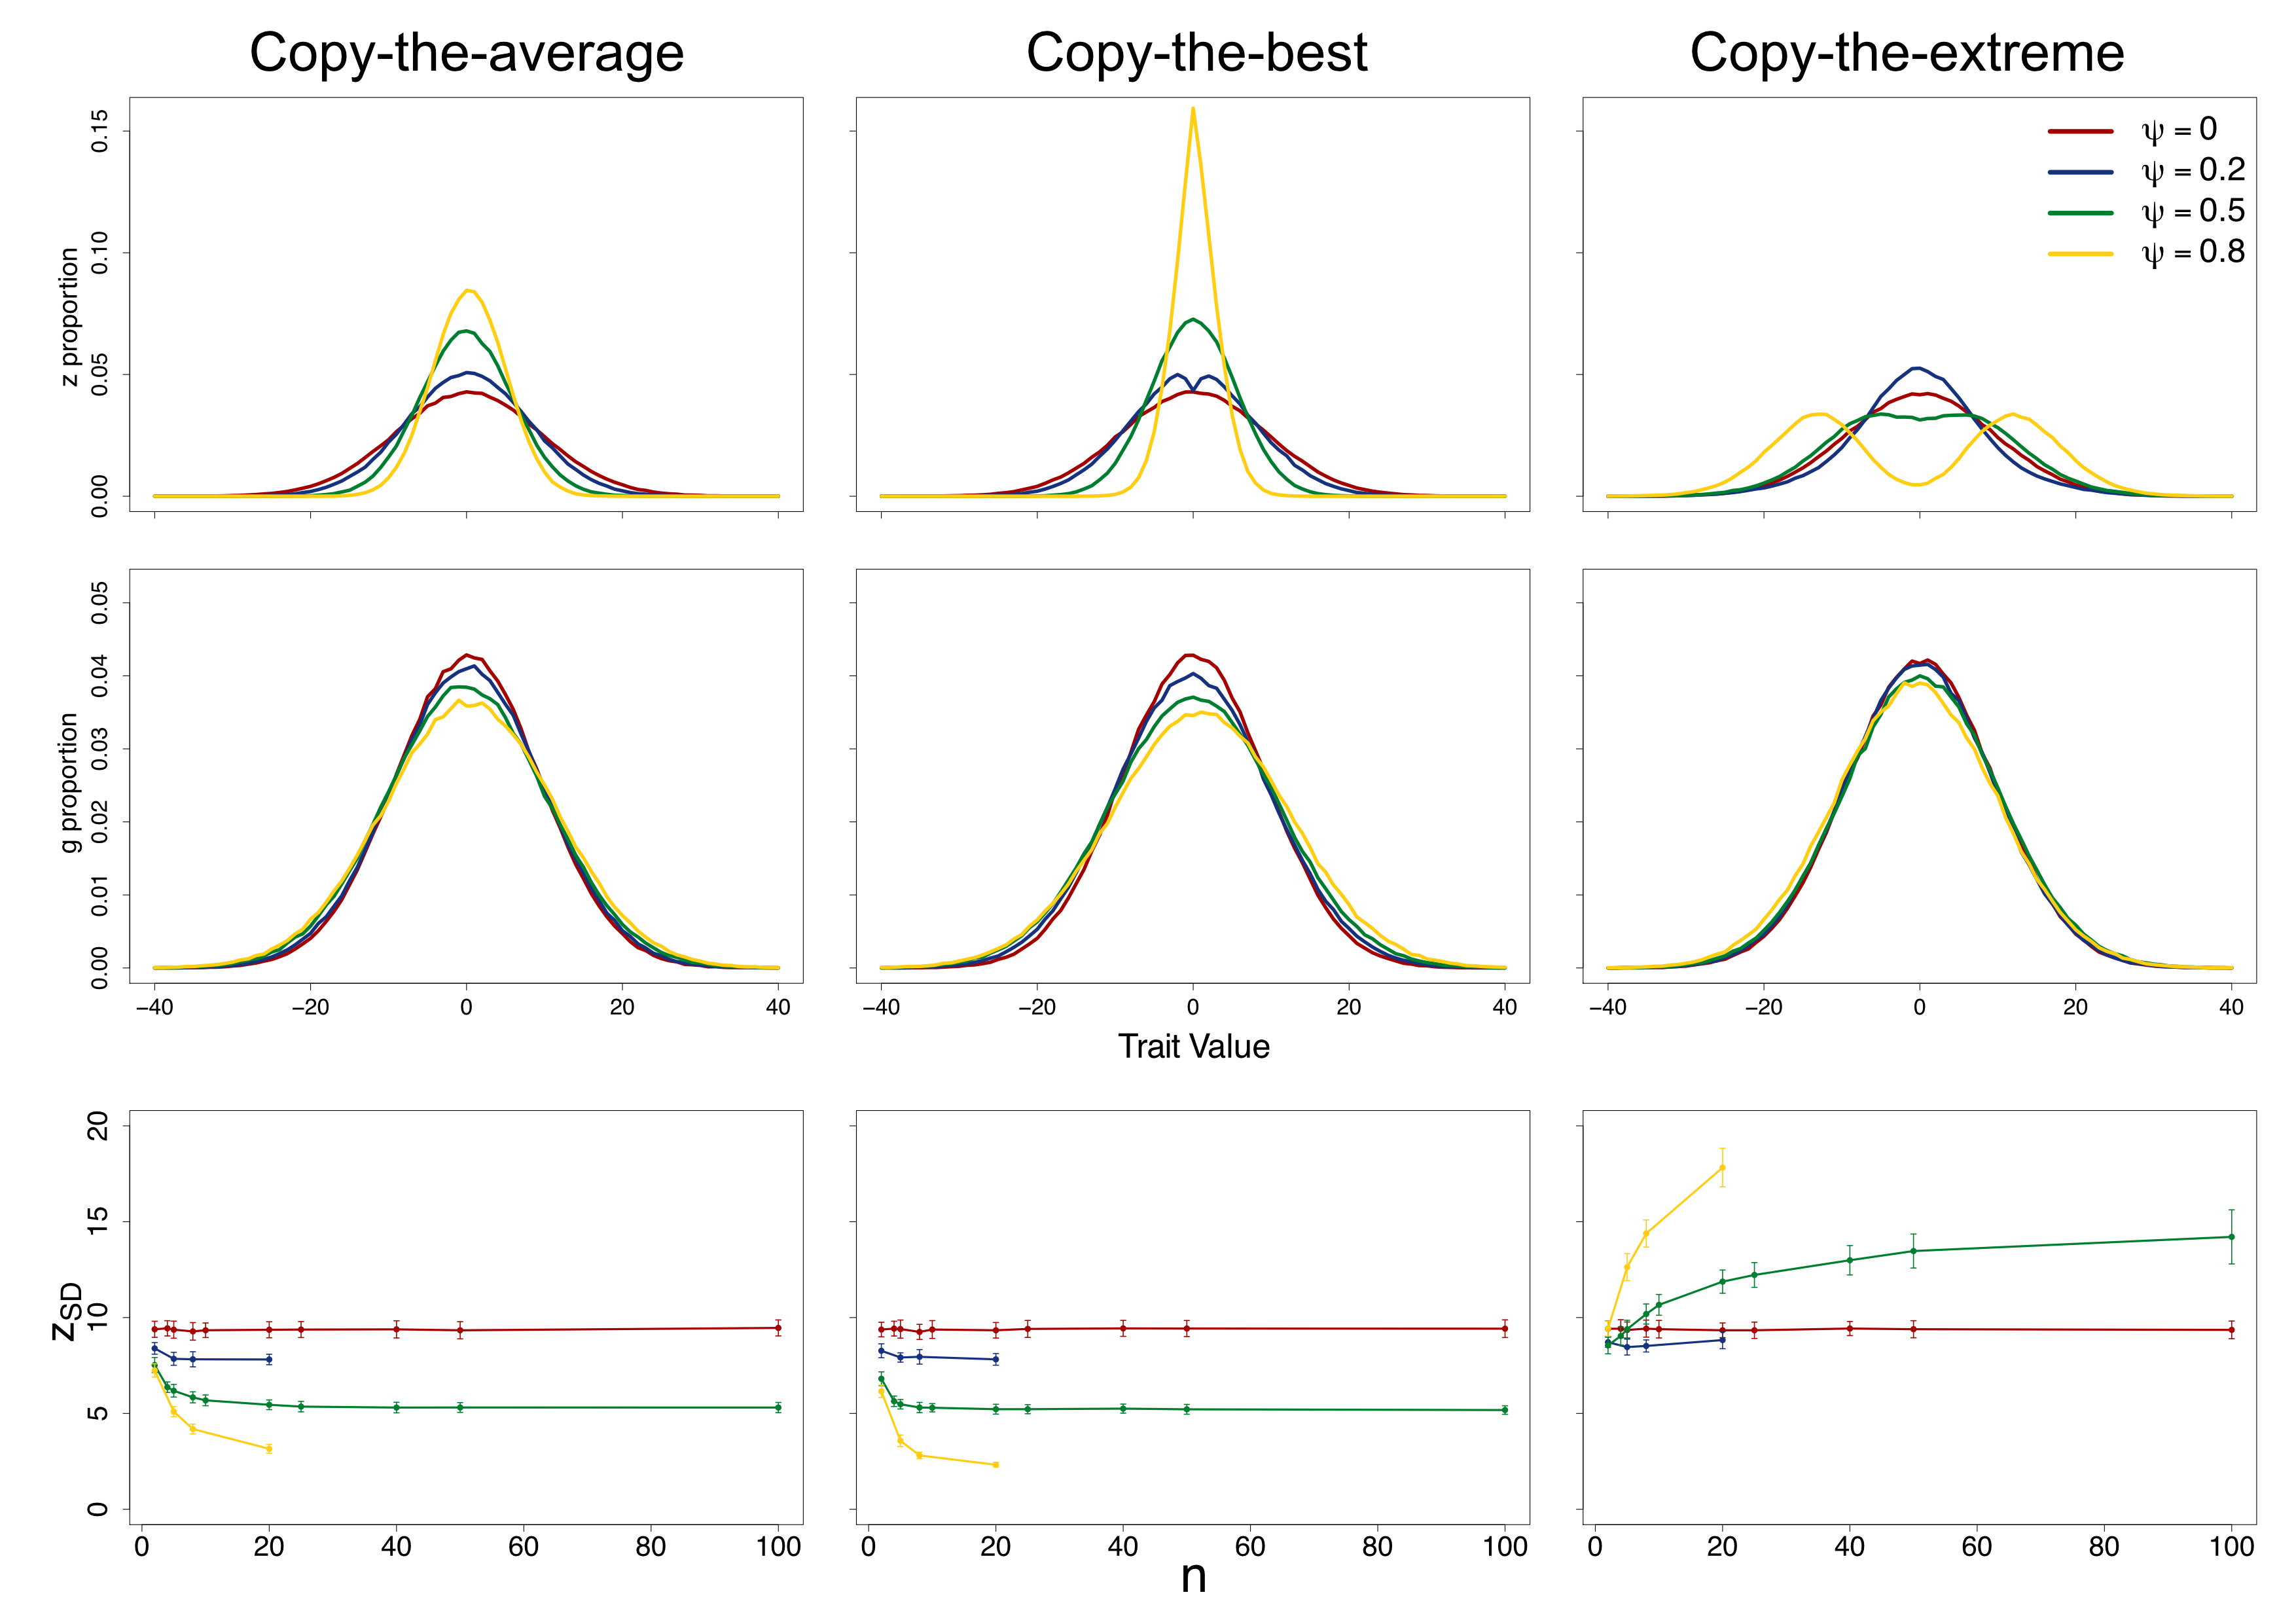
\includegraphics[width=\linewidth]{fig/stab/stab_sel.png}
    \caption{\textbf{Effect of social learning mechanisms, $\psi$, and $n$ on population's statistics under stabilizing selection.} $n=8$ for the top two rows. \textbf{Top row:} Phenotype distribution of different values of $\psi$. For both copy-the-average and copy-the-best model, increasing in $\psi$ always leads to decrease in phenotypic variance. Copy-the-best has slight bimodality for low $\psi$, though the pattern is not significant (see Supplement TODO). Variance for Copy-the-extreme decreases first before increasing as $\psi$ increases, eventually leads to bimodal phenotypic distribution.
    \textbf{Middle row: }Genotypic distribution for different $\psi$. The genotypic variance always increase with $\psi$ regardless of the shape of the phenotypic distribution, though the change is small compare to the change in phenotypic distribution as $\psi$ increasing. 
    \textbf{Bottom row: }Standard deviation (SD) of the phenotypic distribution as a function of group size $n$. For copy-the-average and copy-the-best models, as group size increases, the phenotypic variance further decreases. For copy-the-extreme, higher $n$ leads to a larger distance between modes for larger $\psi$, thus SD is elevated. In all cases, the change in SD decreases as $n$ increases.}
    \label{fig:stabl_sel_1}
\end{figure}
We first examined how different social interaction rules alter the genotype–phenotype relationship under long-term stabilizing selection (Fig \ref{fig:stabl_sel_1}). In the absence of environmental change, all populations evolved around a single fitness optimum, but the shape of the phenotypic distribution depended strongly on both the social rule and the strength of interaction $\psi$. Across all three models, the underlying genotypic distributions remained approximately unimodal and centered near the optimum, indicating that social interactions primarily modified phenotype expression rather than producing large shifts in the population mean genotype. However, the resulting phenotypic distributions differed substantially among social strategies.

Under the copy-the-average model, increasing $\psi$ reduced phenotypic variance (Fig \ref{fig:stabl_sel_1})and slightly increased the genotypic variance (Fig supplement maybe). As individuals placed greater weight on the mean phenotype of their social partners, phenotypes became increasingly concentrated around the population mean. This effect was strengthened by larger group size: as n increased, the social value, $g_{social}$, approached the population mean more closely, causing stronger compression of the phenotypic distribution. Thus, copy-the-average acted as a stabilizing social mechanism that reduced among-individual phenotypic variation while leaving the genotypic distribution comparatively broad.

A similar reduction in phenotypic variance was observed under copy-the-best for small to medium $\psi$ ($\psi < 0.5$) and a much stronger effect for higher $\psi$. As $\psi$ increased, phenotypes became concentrated near the optimum, producing a narrow peak in the phenotypic distribution similar to copy-the-average. This occurs because the copied genotype is chosen based on highest fitness, which under stabilizing selection corresponds to the genotype closest to the optimum. Consequently, social influence under copy-the-best directly pulls phenotypes toward the fitness optimum. Although the genotypic distribution showed only modest changes with increasing $\psi$, the phenotypic distribution became much narrower, indicating that copy-the-best can generate adaptive phenotypic canalization without requiring equivalent genetic change. (TODO: check if the change in phenotypic variance is significantly different for copy the best and copy the average. Their phenotypic distribution for $\psi \leq 0.5$ looks very similar.)

In contrast, copy-the-extreme produced a qualitatively different pattern. Counterintuitively, at lower values of $\psi$, phenotypic variance was slightly reduced relative to the non-social baseline. This non-monotonic pattern arises because, when $\psi$ is weak, copying an extreme group member often pulls individuals only slightly away from their own genotype, and the copied extreme value is still drawn from a distribution centered near the optimum. As a result, $g_{social}$ can reduce moderate deviations before becoming strong enough to amplify tail values. We provide a more comprehensive explanation of this transition in Supplementary Fig. X.

As $\psi$ increases, the phenotype distribution produced by copy-the-extreme became increasingly broad and eventually bimodal. This reflects the fact that individuals copy the group member whose genotype deviates most strongly from the group mean. Under stabilizing selection, such individuals are often located away from the optimum, so stronger social influence shifts phenotypes away from the center of the distribution. The effect increased with group size because larger groups are more likely to contain individuals with more extreme genotypes. As a result, copy-the-extreme amplified phenotypic variance even though the genotype distribution remained approximately normal. (NOTE: could add in the invasion analysis result in this section)

Together, these results show that the evolutionary consequences of social behavior under stabilizing selection depend strongly on the rule by which social information is used. Copy-the-average and copy-the-best both reduce phenotypic variance, but through different mechanisms: copy-the-average pulls individuals toward the group mean, whereas copy-the-best pulls individuals toward the locally highest-fitness genotype. Copy-the-extreme, by contrast, can transform a unimodal genotype distribution into a unimodal or bimodal phenotype distribution depending on strength of interaction $\psi$, demonstrating that social interaction can generate phenotypic structure not directly present in the underlying genetic variation.

\subsection{Directional Selection}
\begin{figure}
    \centering
    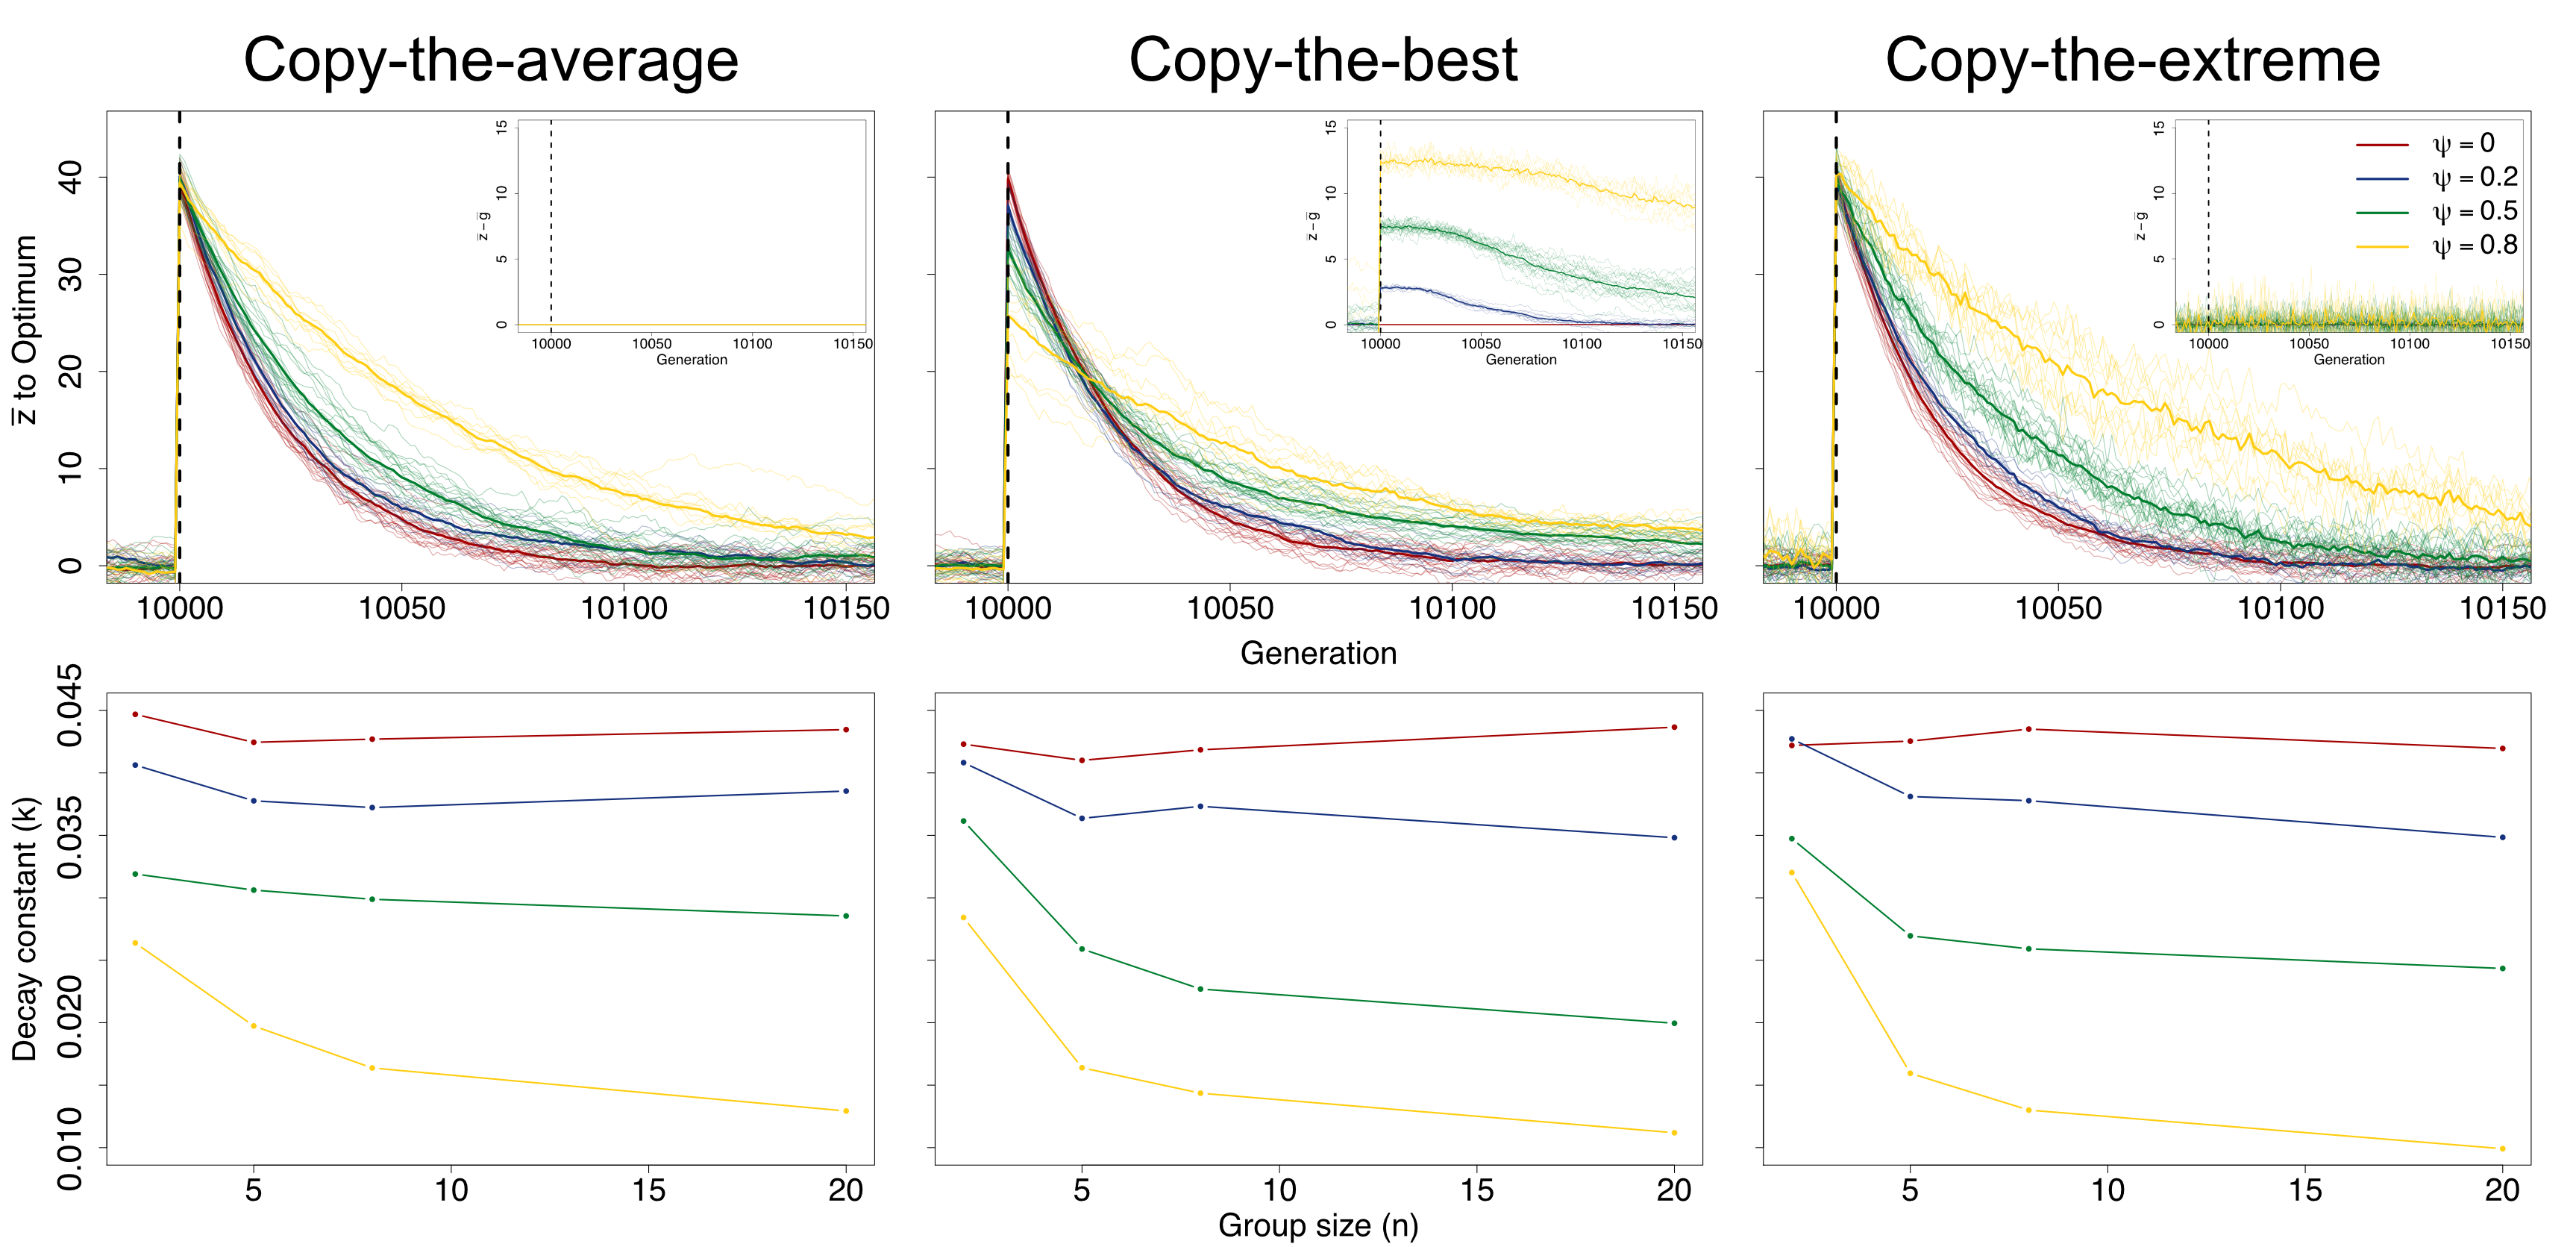
\includegraphics[width=\linewidth]{fig/direc/direc_sel_w_inset_2.png}
    \caption{\textbf{Population adapts to the new optimum after long-term stabilizing selection.} Colored lines represent different interaction strength, $\psi$, with thin lines showing individual simulations and thick lines showing replicate means. $\Lambda=40$ for all simulations shown. \textbf{Top row: } Distance between $\bar{z}$ and the current fitness optimum. After the change at the 10000 generation, all population using copy-the-average and copy-the-extreme is $\Lambda$ unit away from the new optimum. Copy-the-best shows instant phenotypic response, generating $\bar{z}$ that's much closer to the optimum than non-social population ($\psi=0$). Such change in phenotype increases as $\psi$ increases. Inset: mean genotype $\bar{g}$ vs mean phenotype $\bar{z}$ over time. Lighter color is earlier in adaptation. For copy-the-average, $\bar{g}$ tracks $\bar{z}$ perfectly, which is why there's only the yellow points. The tracking is more noisier for copy-the-extreme. Copy-the-best show the largest gap between $\bar{g}$ and $\bar{z}$ earlier in the adaptation and only gets smaller when the phenotype is close to the new optimum. (TODO: change to no replicate lines)
    \textbf{Bottom row: } The decay constant fitted to the line of $\bar{z}$ to new optimum as a function of $n$. As $n$ increases, the rate of approaching the new optimum becomes slower. The change in adaptation rate decreases as $n$ get large, though which $n$ does the plateau reached depends on $\psi$.} 
    \label{fig:direc_sel_1}
\end{figure}

We next asked how social interactions affect adaptation after an abrupt environmental shift. After the population reached mutation–selection–drift balance under stabilizing selection, the fitness optimum was shifted by magnitude $\Lambda$. We then tracked the distance between the population mean phenotype, $\bar{z}$, and the new optimum through time (Fig \ref{fig:direc_sel_1}).

In the non-social baseline, $\psi=0$, the population adapted gradually toward the new optimum through genetic evolution. Copy-the-average and copy-the-extreme showed no immediate phenotypic response at the time of the environmental shift; immediately after the shift, populations remained approximately $\Lambda$ units away from the new optimum. Their subsequent approach toward the optimum was gradual and approximately exponential. However, increasing $\psi$ slowed this recovery, especially at larger group sizes. Under copy-the-average, stronger social influence caused individuals to remain closer to the group mean, reducing the expression of phenotypic deviations in the direction of the new optimum. As a result, higher $\psi$ lowered the decay constant $k$, indicating slower movement toward the optimum.

Copy-the-best showed a distinct short-term response. Immediately after the optimum shifted, populations with stronger social influence produced mean phenotypes closer to the new optimum than the non-social baseline. This immediate response occurred because the best genotype in each group was now biased toward the new optimum, allowing individuals to express phenotypes closer to the new selective target before the population mean genotype had evolved substantially. The magnitude of this response depended on $\psi$ and $n$, where increasing either of these parameters increases the response as a result of increased genetic variation under stabilizing selection (Fig TODO: heatmap of the jump, maybe in supplement). A larger genetic reservoir means that more low-fitness individual was retained under stabilizing selection; they subsequently became the high-fitness leader of their group when the shift happened. Thus, copy-the-best generated an initial adaptive plastic response and the response is dependent on the interaction strength and group size. 

However, this short-term benefit did not necessarily translate into faster long-term adaptation. After the initial phenotypic jump, populations with $\psi\neq 0$ often approached the optimum more slowly than the non-social baseline. The decay constant decreased with increasing $\psi$ and with increasing group size, suggesting that strong social influence can partially shield genetic variation from selection by reducing the direct relationship between an individual’s genotype and expressed phenotype. This is also visible in the difference between mean genotype and mean phenotype over time: early after the shift, $\bar{z}$ are roughly 12 units ahead of $\bar{g}$. Such gap gradually decreases as genetic evolution catches up with phenotypic evolution because of relaxed selection on phenotypes as the population approaches the new optimum. In other words, copy-the-best can produce adaptive plasticity in the short term while slowing genetic tracking of the new optimum over longer timescales, and the trade-off is $\psi$ and $n$ dependent.

Copy-the-extreme also slowed adaptation after the environmental shift. Similar to copy-the-average, it did not generate a strong adaptive jump toward the new optimum. Instead, stronger social influence increased phenotypic spread and introduced noisier tracking between genotype and phenotype. This reduced the efficiency with which selection acted on genetic values aligned with the new optimum. As with the other mechanisms, increasing group size generally reduced the estimated decay constant, with the effect becoming weaker at larger n, suggesting a plateau in the influence of group size.

Overall, social rules altered both the immediate phenotypic response to environmental change and the subsequent rate of adaptation. Copy-the-best was unique in producing a rapid adaptive shift in phenotype immediately after the environment changed, but all three social mechanisms tended to reduce the long-term rate of approach to the new optimum when social influence was strong. The pattern for copy-the-best is expected from previous studies in phenotypic plasticity (citation needed) and social plasticity (\cite{Martin2025}). These results indicate that the mechanism of how social plasticity is generated can have impact on the population's adaptation even if all three models generated similar genotype-phenotype mismatch under stabilizing selection. 

\subsection{Fluctuating Environment}

\begin{figure}
    \centering
    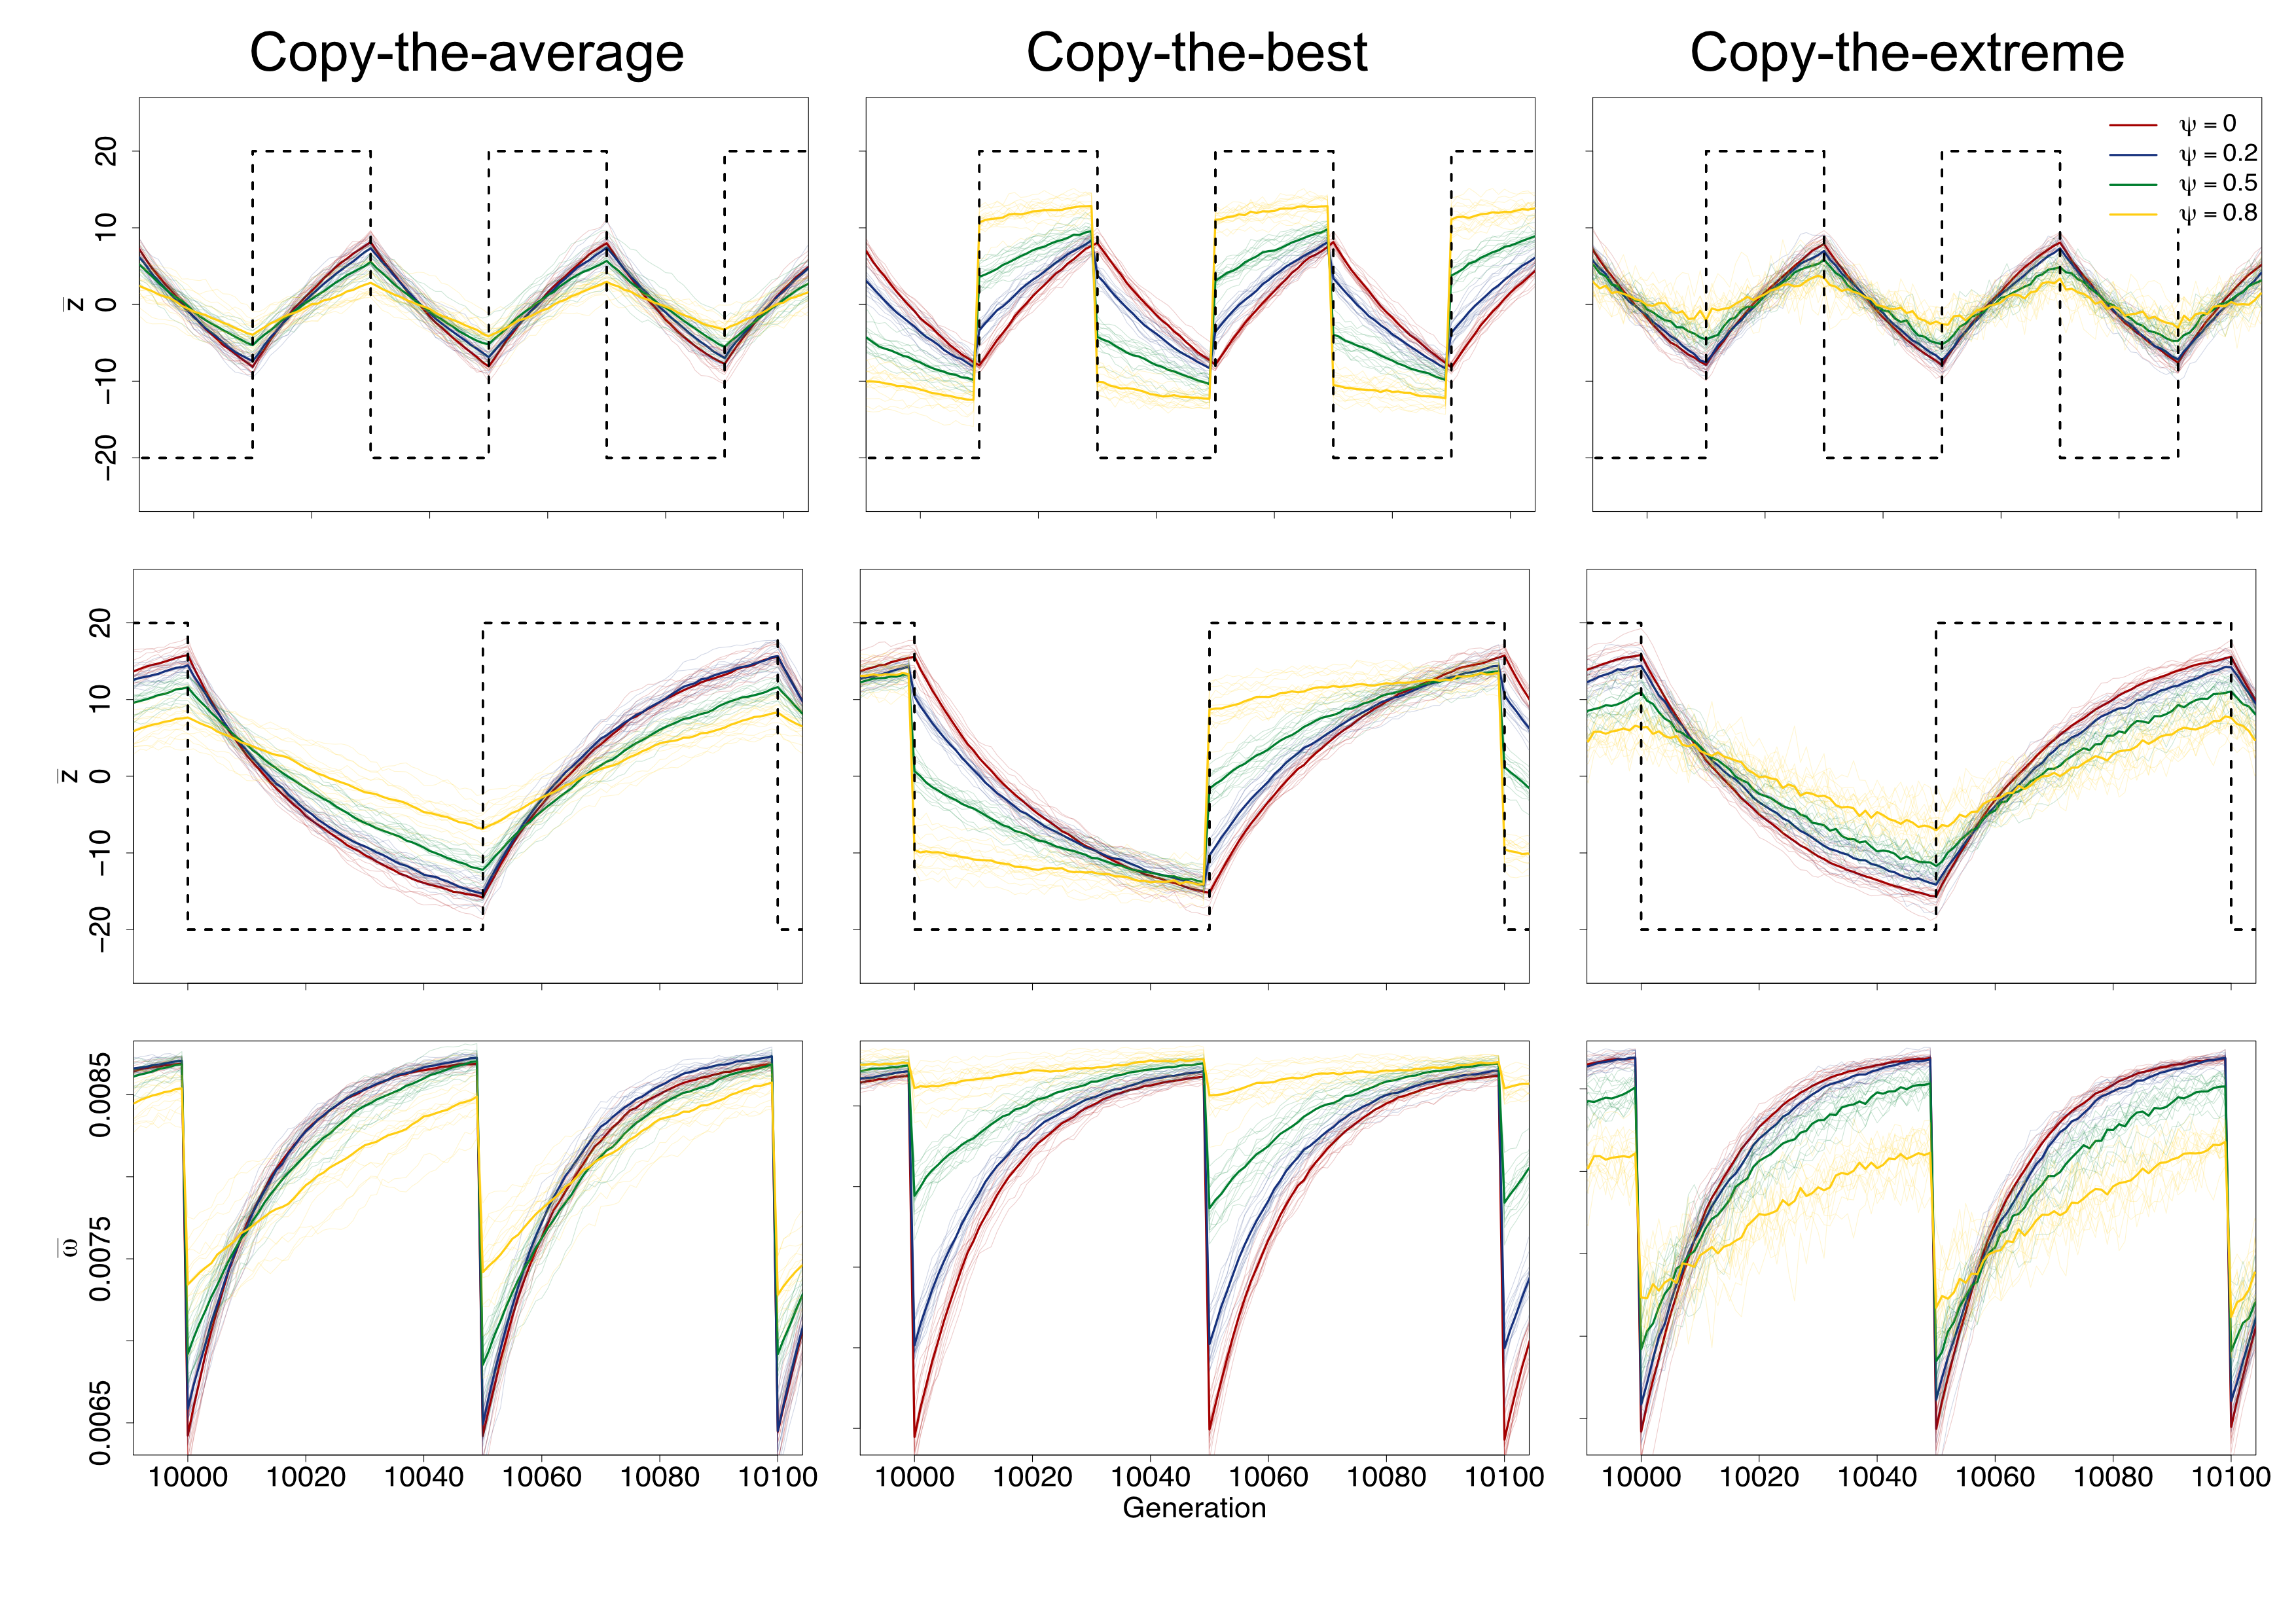
\includegraphics[width=\linewidth]{fig/fluc/fluc_env_main.png}
    \caption{\textbf{Models track the optimum differently under a periodically fluctuating environment.} Population responses are shown under three social learning rules: copy-the-average, copy-the-best, and copy-the-extreme. Black dashed lines indicate the environmental optimum. \textbf{Top and middle row:} The phenotypic mean of the population over time with different frequency $f$. $f=\frac{1}{40}$ generations and $f=\frac{1}{100}$ generations for the top row and middle row, respectively. \textbf{Bottom row:} population mean fitness $\bar{\omega}$ for the middle row.}
    \label{fig:fluc_env_main}
\end{figure}

\begin{figure}
    \centering
    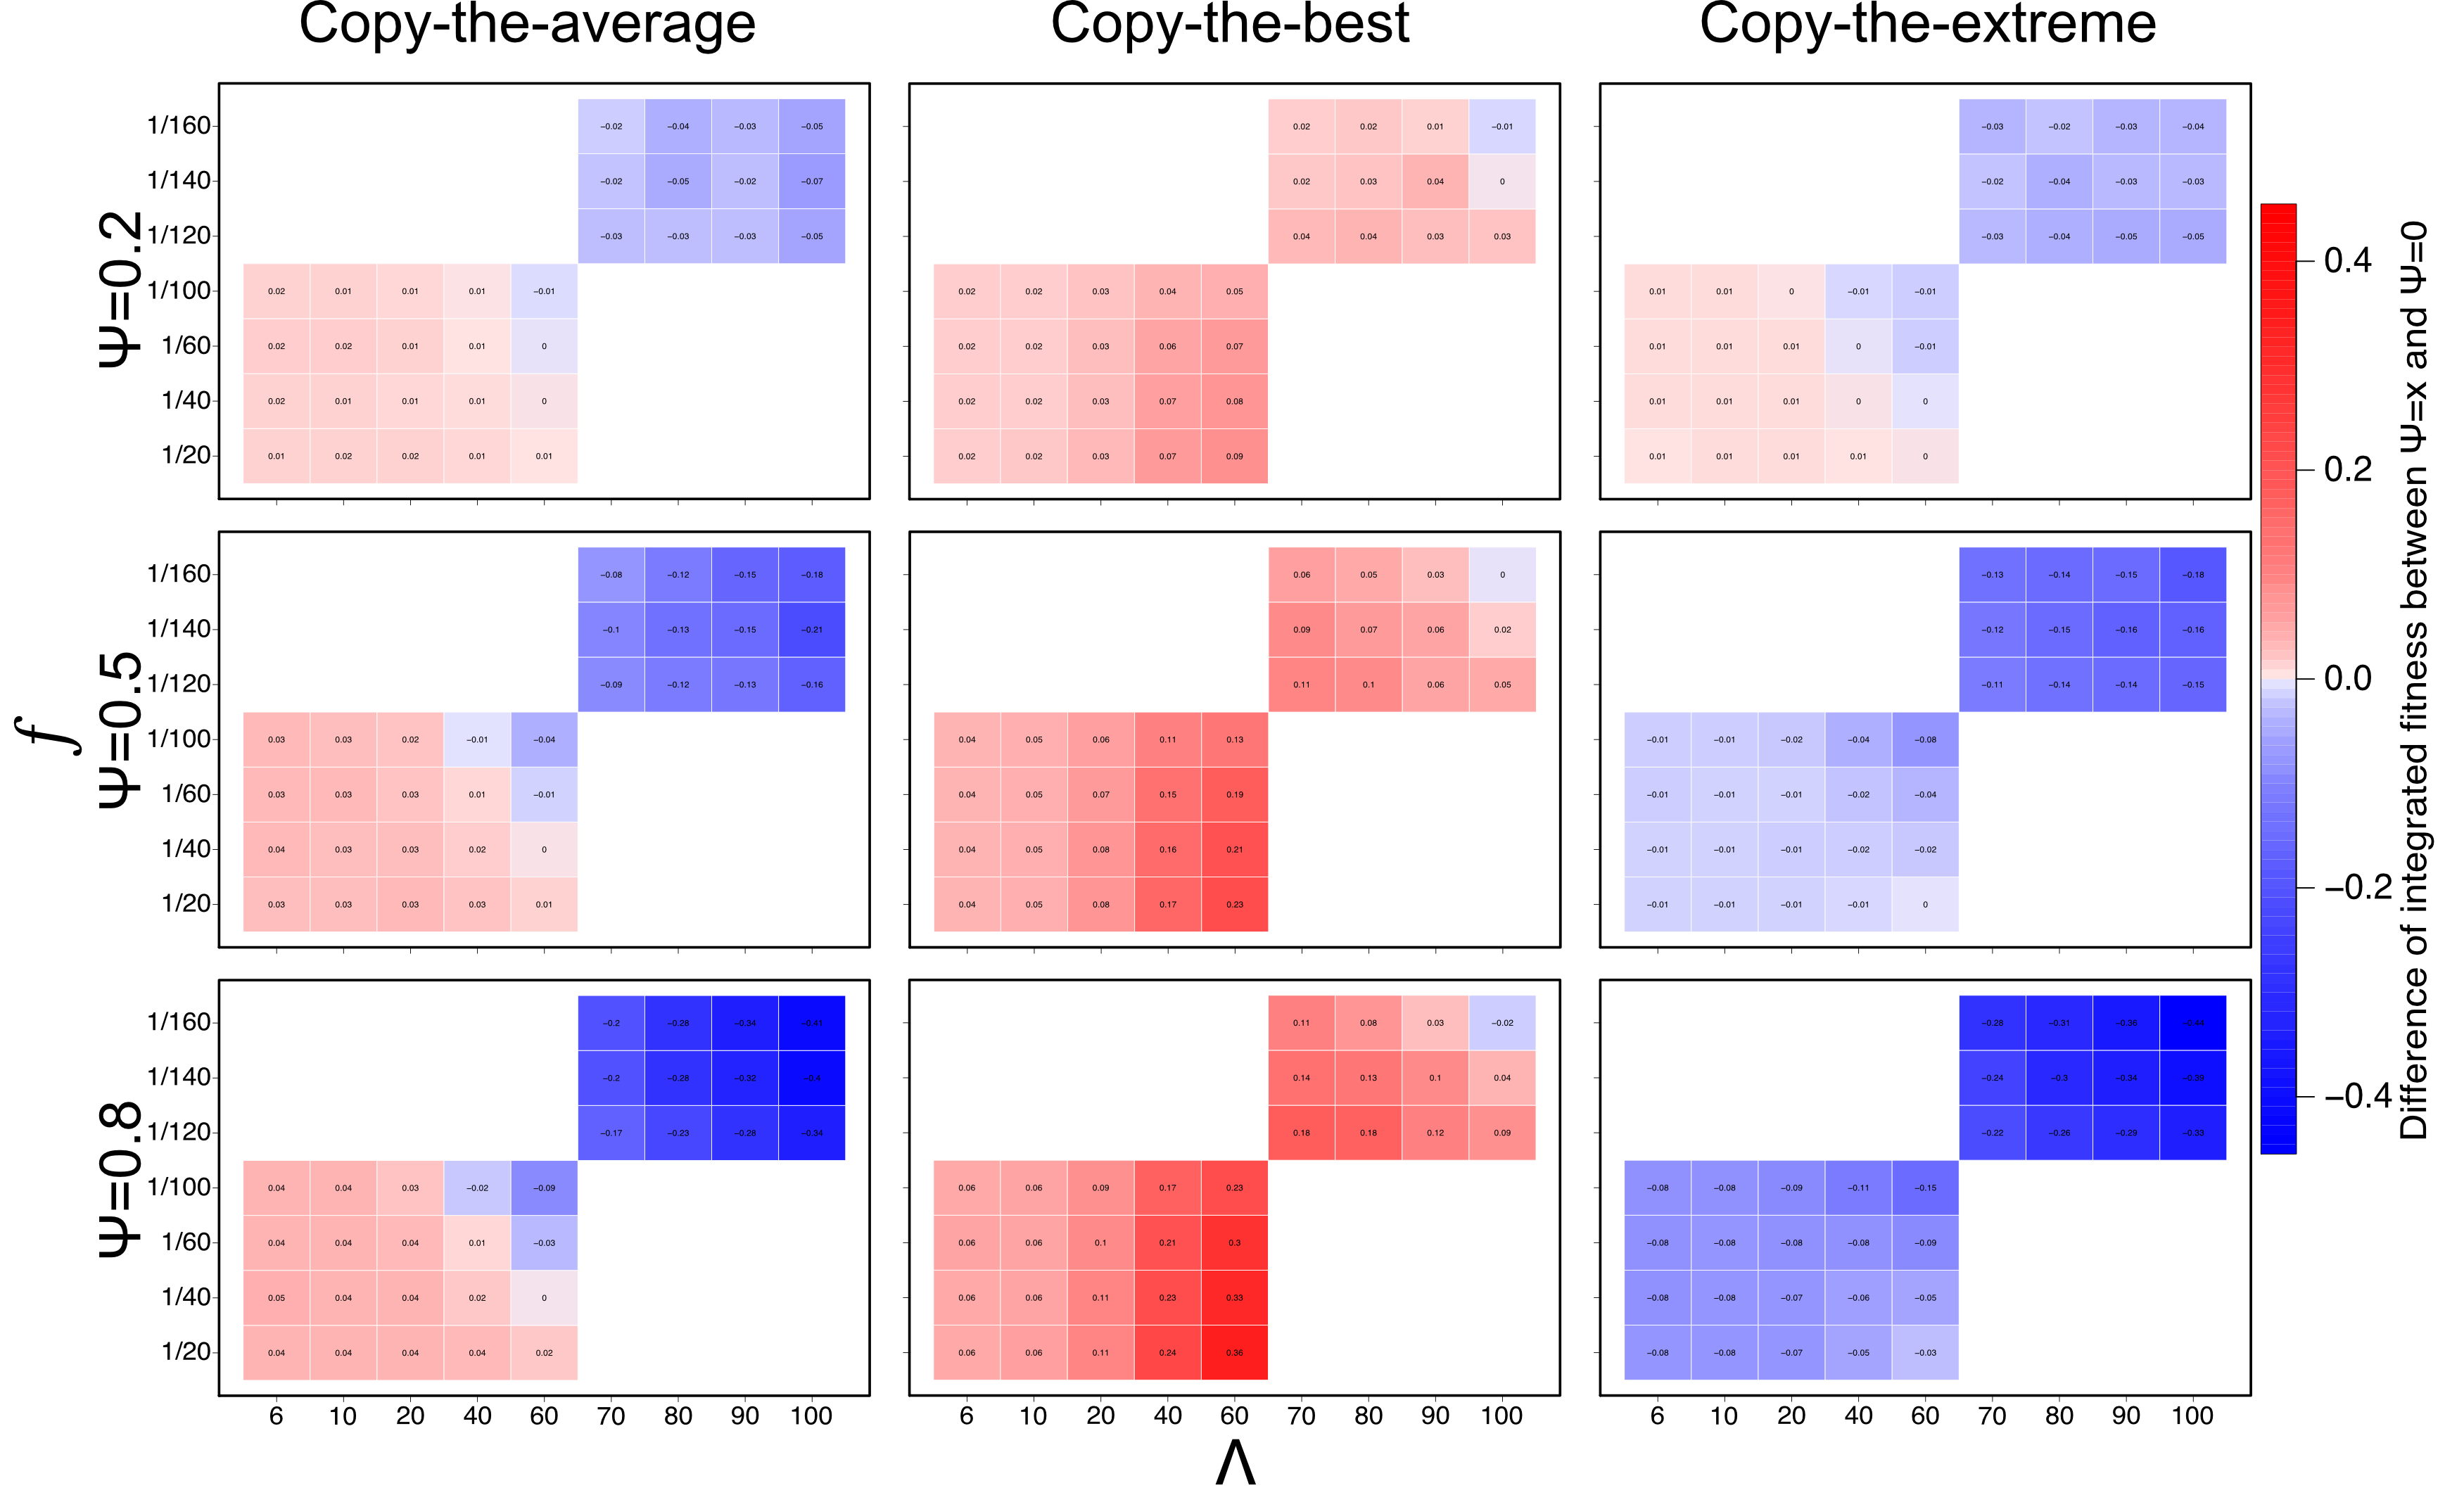
\includegraphics[width=\linewidth]{fig/fluc/integrated_fitness_fluc_env.png}
    \caption{\textbf{Integrated fitness differences across fluctuating environments.} Each tile shows the replicate-averaged difference in cumulative mean fitness between a social population and the corresponding non-social baseline, $\psi=0$, after summing $\bar{\omega}$ across 300 generations. Red indicates that social behavior produced higher integrated fitness than the $\psi=0$ baseline, while blue indicates lower integrated fitness. Copy-the-best generally improves cumulative fitness across much of the parameter space, especially at larger $\psi$ and moderate shift sizes. Copy-the-average and Copy-the-extreme can yield higher cumulative fitness when environmental shifts are small or infrequent, though the reduction in fitness is more severe otherwise.}
    \label{fig:fluc_env_fit}
\end{figure}

Finally, we examined how populations respond when the fitness optimum fluctuates periodically between two trait values. This regime differs from the single-shift scenario because the direction of selection repeatedly changes before the population fully reaches either optimum through constrains in the value of $f$ tested. We therefore asked whether social interaction improves or worsens tracking of a moving optimum, and whether the effect depends on fluctuation frequency, shift size, group size, and social strategy.

Across all models, populations lagged behind the changing optimum (Fig \ref{fig:fluc_env_main}). However, the magnitude and direction of this lag depended on the social rule. Under copy-the-average, increasing $\psi$ reduced the amplitude of phenotypic tracking. This damping could be beneficial when environmental changes were frequent or small. The population adapts slower to one optimum, which means the population is closer to the other optimum when the optimum shifts compared to the non-social population which adapts faster. However, the benefit of lagging behind only lasted a few generations before the non-social population outperforms all social populations. Thus, even though copy-the-average has the fitness advantage over non-social model, the benefit is dependent on how environment fluctuates, namely $f$ and $\Lambda$.

To investigate the effect of $f$ and $\Lambda$ on the fitness outcome of each model, we integrated $\bar{\omega}$ for each simulation and looked at how do $f$ and $\Lambda$ affect whether a certain parameter set is better than the non-social population (Fig \ref{fig:fluc_env_fit}). For copy-the-average, the population has a higher overall fitness when $f$ or $\Lambda$ is small. As either of them increases, the social population's fitness decreases. For a larger $\psi$, the fitness benefit at low $f$ or $\Lambda$ is higher, but the reduction is also more severe when either of the parameters increases. 

Copy-the-best generated a different form of tracking. At each environmental shift, the abrupt phenotypic responses allowed populations to move toward the new optimum more quickly than expected from genetic change alone in short time (Fig \ref{fig:fluc_env_main}). However, the slower adaptation following the plastic response limited population's optimum tracking when the frequency is lower. The non-social baseline population was able to catch up after some time and its $\bar{z}$ became closer to the  optimum than that of social populations. Therefore, whether copy-the-best is beneficial depended on the value of $f$ and $\Lambda$ combined.

When looked at the integrated fitness, copy-the-best generally produced higher cumulative $\bar{\omega}$ than the non-social baseline across much of the parameter space, especially at moderate shift sizes and higher $\psi$ (Fig \ref{fig:fluc_env_fit}). This suggests that fitness-biased social learning can be beneficial in fluctuating environments because it allows phenotypes to respond plastically to the currently favored direction of selection. However, this advantage diminished when $f$ or $\Lambda$ deviates from moderate level. For small $\Lambda$, non-social baseline could track the optimum well enough that its integrated fitness was close to that of a social population. On the other hand, when $\Lambda$ was large and $f$ was small, the social population is maladaptive where the fitness drawback of the slower adaptation outweighs the benefit from the initial plastic response.

Copy-the-extreme generally reduced tracking accuracy in fluctuating environments and behaved similarly to copy-the-average. Because individuals copied the most extreme genotype in the group rather than the genotype closest to the current optimum, social influence often pushed phenotypes away from the optimal value. This effect became especially costly at large shift sizes and high $\psi$, where integrated fitness was substantially lower than in the non-social baseline. Under some mild environmental conditions, such as small shifts and frequent fluctuations, copy-the-extreme could have weakly positive or near-neutral effects, but its overall effect was more often negative than copy-the-best.

Across the three selection regimes, social interaction had context-dependent evolutionary effects. Under stabilizing selection, social behavior often increased population performance by reducing maladaptive phenotypic variance, except when social influence favored extreme group members with medium to high interaction strength. After a single environmental shift, social behavior could generate rapid plastic responses under copy-the-best, but strong social influence generally slowed longer-term adaptation. In fluctuating environments, the benefit of sociality depended on whether the social rule helped individuals track the currently favored phenotype. Thus, the same social mechanism that is beneficial in a stable environment can become costly under directional or fluctuating selection, depending on how it reshapes the genotype–phenotype map.

% \newpage
% \section{Discussion}

% copy the best behave like what people predict under regular phenotypic plasticity. a quick response first but then a slower adaptation later. the other two strategies are also justified biologically, though they don't produce the expected pattern for plasticity. this means that social plasticity might be a special case and the mechanism of how social plasticity is generated has big impact on the evolutionary consequences for the population.

% group size in our model should not be interpreted as group size in literal sense. our model assumes all-to-all relationship among individuals, where in reality individuals tend to only pay attention to the individuals around them even if they are in a huge group. therefore the group size might be huge on paper but the effective group size is not going to be comparable.

% find some literature/biological studies on how learning happens and what rules do individuals use to choose the individual to learn. 

% we have feedback loop in copy the average, yet it just constrains the population to one state rather than generating run away phenotypes. on the other hand, copy the best doesn't have feedback loop, yet it behave the most like a adaptive phenotypic plasticity. 

% chat: The runaway effect in the original Moore et al. formulation is biologically meaningful when social interactions are amplifying, such as aggression, display, panic, or social contagion. However, for social learning or social plasticity where individuals integrate social information with their own tendency, a convex-combination model is more appropriate because social influence replaces part of the individual contribution rather than being added independently.



% % \lipsum[2-4]

% \newpage


% \paragraph{copy-the-Best}

% \subsection{Selection Regime}
% \paragraph{Fitness function}

% % Viability selection acted on the expressed phenotype through a Gaussian fitness function,
% % \begin{equation}
% % w_i = \exp\!\left[-\frac{(z_i - \theta)^2}{2V_s}\right],
% % \end{equation}
% % where $\theta$ denotes the current phenotypic optimum and $V_s$ determines the strength of stabilizing selection. Fitness values were applied directly as individual fitness-scaling factors, and population size was regulated by Wright--Fisher reproduction.

% \paragraph{Dynamics of the phenotypic optimum}
% There are two types of selection regime we have tested. 
% First, the optimum may shift once at a specified generation $t_{\mathrm{shift}}$, representing an abrupt environmental change \cite{Hayward2022}. The magnitude of the shift, $\Delta \theta$, is a parameter. Under this regime, the optimum is constant before and after the shift.
% Second, the optimum may fluctuate periodically between two values at fixed intervals. In this regime, the amplitude and the interval of the fluctuation, TODO:VARIABLE, are explicit parameters of the model. The optimum alternates deterministically between states.

% % Together, these alternative schedules allow direct comparison between evolutionary responses to sustained directional selection and to recurrent environmental fluctuations, while holding demographic structure and genetic architecture constant.






% \section{Analytical Analysis}
% \subsection*{Rare–Mutant Invasion Under Extreme Copying}

% % We consider a resident population of asocial individuals ($\psi=0$), where direct genotypes are i.i.d. draws from a normal distribution,
% % \[
% % a \sim \mathcal{N}(\mu, V),
% % \]
% % and phenotypes equal genotypes. A rare mutant with copying strength $\psi \in (0, 1]$ enters this population. Individuals form random groups of size $n$, and the mutant applies the copy-extreme rule: it replaces a fraction $\psi$ of its own genotype with that of the resident individual whose genotype is furthest from the group mean. Throughout this section we consider only the case in which the individual identified as the extreme is a \emph{resident}; the probability that the rare mutant is the extreme is $\frac{1}{n}$ and contributes only a term of order $1/n$, which is negligible in the rare–mutant limit. In addition, the mutant is practically asocial if it self-copies. 

% % \paragraph{Model.}
% % Let $A$ denote the direct genotype of the mutant and $g_1,\dots,g_{n-1}$ the genotypes of the resident group members.  The group mean is
% % \[
% % \bar a = \frac{A + \sum_{j=1}^{n-1} g_j}{n}.
% % \]
% % Define the resident $j^*$ whose genotype is most distant from the mean,
% % \[
% % j^* = \arg\max_{j \in \{1,\dots,n-1\}} |g_j - \bar a|,
% % \qquad
% % E := g_{j^*}.
% % \]
% % The mutant phenotype is
% % \[
% % z_m = (1-\psi) A + \psi E.
% % \]
% % Residents retain $z=a$.

% % \paragraph{Distribution of the resident extreme.}
% % Let $g_j$ be standardized and $g_j = \mu + \sqrt{V}\,Y_j$ with $Y_j \sim \mathcal{N}(0,1)$. Neglecting the small difference between $\bar a$ and $\mu$ under the assumption that the population has been under stabilizing selection and $\mu=\bar{z}$, the distribution of $E$ depends on the ``two-sided'' extreme
% % \[
% % S := \max_{1 \le j \le n-1} |Y_j|.
% % \]

% % It is well known that the maximum of $m$ independent standard normal variables lies in the domain of attraction of the Gumbel extreme-value distribution.  In particular, letting $M_m = \max(Y_1,\dots,Y_m)$, there exist constants $g_m>0$ and $b_m$ such that
% % \[
% % \frac{M_m - b_m}{g_m} \;\Rightarrow\; G,
% % \]
% % where $G$ has a standard Gumbel distribution. For normal variables one may take $b_m \approx \sqrt{2\ln m}$ and $g_m \approx \frac{1}{\sqrt{2\ln m}}$. Since $S = \max(M_{n-1}, -\min(Y_1,\dots,Y_{n-1}))$, symmetry implies that $E$ is approximately symmetric around $\mu$ and has variance
% % \begin{equation}
% %     \operatorname{Var}(E)
% %     \;\approx\;
% %     V_{\rm ext}
% %     := 2V \ln(n-1).
% % \end{equation}
% % Thus, for our purposes,
% % \[
% % \mathbb{E}[E] = \mu,
% % \qquad
% % \operatorname{Var}(E) = V_{\rm ext}.
% % \]

% % \paragraph{Mutant phenotype distribution.}
% % Since $A$ and $E$ belong to disjoint sets of individuals, they are independent in the rare–mutant limit.  Therefore
% % \[
% % \mathbb{E}[z_m]
% % = (1-\psi)\mu + \psi \mu
% % = \mu.
% % \]
% % The variance follows from independence:
% % \[
% % \operatorname{Var}(z_m)
% % = (1-\psi)^2 \operatorname{Var}(A)
% %   + \psi^2 \operatorname{Var}(E)
% % = (1-\psi)^2 V + \psi^2 V_{\rm ext}.
% % \]
% % Expanding around $\psi=0$,
% % \begin{equation}
% %     V_{\rm mut}(\psi)
% %     = V - 2V\psi + \psi^2(V + V_{\rm ext}).
% %     \label{eq:Vmut_expansion}
% % \end{equation}
% % Thus, to \emph{first order} in $\psi$, the mutant exhibits reduced 
% % phenotypic variance relative to residents.  
% % The influence of the extreme tail (i.e.\ the Gumbel term 
% % $V_{\rm ext}$) appears only at order $\psi^2$.

% % \paragraph{Mean fitness and invasion condition.}
% % Under Gaussian stabilizing selection,
% % \[
% % W(z)
% % = \exp\!\left( -\frac{(z-\theta)^2}{2\sigma_w^2} \right),
% % \]
% % individuals with normally distributed phenotypes and mean equal to 
% % the optimum ($\mu=\theta$) have mean fitness
% % \[
% % \bar W(V_z)
% % = \frac{1}{\sqrt{1 + V_z/\sigma_w^2}}.
% % \]
% % Since residents have variance $V$, 
% % \[
% % \bar W_{\rm res}
% % = \frac{1}{\sqrt{1 + V/\sigma_w^2}},
% % \qquad
% % \bar W_{\rm mut}(\psi)
% % = \frac{1}{\sqrt{1 + V_{\rm mut}(\psi)/\sigma_w^2}}.
% % \]

% % Define the invasion fitness
% % \[
% % s(\psi)
% % = \ln\!\left(
% %     \frac{\bar W_{\rm mut}(\psi)}
% %          {\bar W_{\rm res}}
% %   \right)
% % = -\frac{1}{2}
% %   \ln\!\left(
% %     \frac{\sigma_w^2 + V_{\rm mut}(\psi)}
% %          {\sigma_w^2 + V}
% %   \right).
% % \]
% % Differentiating and evaluating at $\psi=0$ gives
% % \[
% % \left.\frac{ds}{d\psi}\right|_{\psi=0}
% % = -\frac{1}{2}
% %   \frac{1}{\sigma_w^2 + V}
% %   \left.\frac{dV_{\rm mut}}{d\psi}\right|_{\psi=0}.
% % \]
% % From (\ref{eq:Vmut_expansion}),
% % \[
% % \left.\frac{dV_{\rm mut}}{d\psi}\right|_{\psi=0}
% % = -2V,
% % \]
% % and therefore
% % \begin{equation}
% %     \left.\frac{ds}{d\psi}\right|_{\psi=0}
% %     = \frac{V}{\sigma_w^2 + V}
% %     > 0.
% % \end{equation}
% % Hence a rare extreme-copying mutant with sufficiently small $\psi>0$ can 
% % invade an asocial resident population.

% % \paragraph{When is $\psi$ not small?}
% % The evolutionary effect of $\psi$ in the rare-mutant limit depends on whether $\psi$ is sufficiently small for the first-order contribution to the mutant phenotype to dominate, or sufficiently large that nonlinear effects arising from copying extreme phenotypes become important. Here we formalize these two regimes and derive the critical threshold separating them.

% % \subsubsection*{Small--$\psi$ regime}

% % For a mutant with phenotype
% % \[
% % z_m = (1-\psi)A + \psi E,
% % \]
% % where $A$ is the mutant’s own genotype and $E$ is the extreme resident
% % genotype in its group, the resulting phenotype variance is
% % \[
% % V_{\mathrm{mut}}(\psi)
% % = V - 2V\psi + \psi^2\,(V + V_{\mathrm{ext}}),
% % \]
% % with $V$ the resident variance and $V_{\mathrm{ext}} \approx 2V\ln(n-1)$ the variance of the extreme genotype in a group of size $n$.  

% % The \emph{small--$\psi$ regime} is defined by values of $\psi$ for which the first‐order term dominates the quadratic term, i.e.
% % \[
% % 2V\psi \gg \psi^2 (V + V_{\mathrm{ext}}).
% % \]
% % In this range, the mutant experiences a net reduction in phenotypic
% % variance,
% % \[
% % V_{\mathrm{mut}}(\psi) \approx V - 2V\psi,
% % \]
% % and therefore gains higher mean fitness under stabilizing selection.
% % Consequently, any rare mutant with sufficiently small $\psi>0$ can invade.

% % \subsection*{Large--$\psi$ regime}

% % When $\psi$ becomes sufficiently large, the quadratic term in
% % $V_{\mathrm{mut}}(\psi)$ dominates the linear variance‐reducing effect.
% % Since $V_{\mathrm{ext}}$ grows with group size via the extreme‐value
% % scaling $V_{\mathrm{ext}} \approx 2V\ln(n-1)$, the term
% % $\psi^2(V + V_{\mathrm{ext}})$ inflates the mutant’s variance and drives
% % its phenotype far from the fitness optimum. In this \emph{large--$\psi$
% % regime}, selection becomes negative and $\psi$ is no longer favored.

% % \subsection*{Critical threshold \texorpdfstring{$\psi_c$}{psi\_c}}

% % The boundary between the two regimes is obtained by equating the linear
% % and quadratic contributions:
% % \[
% % 2V\psi_c \;=\; \psi_c^2\,(V + V_{\mathrm{ext}}).
% % \]
% % For $\psi_c>0$, this yields
% % \[
% % \psi_c = \frac{2V}{V + V_{\mathrm{ext}}}
% %        = \frac{2}{1 + 2\ln(n-1)},
% % \]
% % where we have substituted $V_{\mathrm{ext}} \approx 2V\ln(n-1)$.  Values
% % $\psi \ll \psi_c$ lie in the small--$\psi$ regime and favor invasion,
% % whereas $\psi \gg \psi_c$ fall in the large--$\psi$ regime and are
% % selected against.

% % \subsection*{Critical values for typical group sizes}

% % \begin{center}
% % \begin{tabular}{c c c}
% % \toprule
% % Group size $n$ & $\ln(n-1)$ & Critical value 
% % $\displaystyle \psi_c = \frac{2}{1 + 2\ln(n-1)}$ \\
% % \midrule
% % 5   & 1.39 & 0.53 \\
% % 10  & 2.20 & 0.37 \\
% % 20  & 2.94 & 0.29 \\
% % 50  & 3.89 & 0.23 \\
% % 100 & 4.60 & 0.20 \\
% % \bottomrule
% % \end{tabular}
% % \end{center}

% % These values illustrate that the variance‐inflation effect of copying
% % extremes becomes strong at relatively small values of $\psi$, especially
% % for large group sizes.



% \section{Result}
% \begin{figure}
%     \centering
%     \includegraphics[width=\linewidth]{fig/geno_pheno_dist.png}
%     \caption{\textbf{Effects of social copying strategies on genotypic and phenotypic trait distributions under stablizing selection.}
% Distributions of genotypes ($a$, top row) and phenotypes ($z$, bottom row) are shown for three social strategies: copy-the-average (left), copy-the-extreme (center), and copy-the-best (right).
% For each strategy, results are compared between the asocial case ($\psi = 0$, red) and strong social influence ($\psi = 0.9$, blue).
% Genotypic distributions are identical across $\psi$ for the copy-the-average and copy-the-extreme strategies, whereas the copy-the-best strategy maintains a broader genotypic distribution when $\psi > 0$.
% In contrast, phenotypic distributions respond strongly to social influence: phenotypic variance is substantially reduced under copy-the-average and copy-the-best, while copy-the-extreme generates high and bimodal phenotypic variation.
% Parameter used: $n=50$.}
%     \label{fig::geno_pheno_dist}
% \end{figure}


% Figure \ref{fig::geno_pheno_dist} compares the distributions of genotypes and phenotypes under stabilizing selection across three social strategies—copy-the-average, copy-the-extreme, and copy-the-best. The comparison focuses on the asocial case ($\psi=0$) and the strong social influence ($\psi=0.9$). Across strategies, genotypic and phenotypic responses to sociality differently. For both the copy-the-average and copy-the-extreme strategies, the genotypic distributions are effectively unchanged by sociality: the distributions under $\psi=0$ and $\psi=0.9$ overlap closely, indicating that social effects act at the phenotypic level without altering the underlying genetic variance. In contrast, under the copy-the-best strategy, the genotypic distribution is significantly wider for $\psi=0.9$, suggesting that socially mediated phenotypes modify the selective environment in a way that increases genetic variance.

% Phenotypic distributions show even stronger contrasts across strategies. Under copy-the-average, increasing $\psi$ leads to a narrowing of the phenotypic distribution, with phenotypes concentrated around the population mean despite standing genetic variation. A similar but more extreme decrease of phenotypic variance is observed under copy-the-best model, where strong social influence produces a peaked phenotypic distribution. By contrast, under copy-the-extreme, phenotypic variance remains high under , and the distribution becomes multimodal, indicating that individuals can express markedly different phenotypes even when drawn from similar or identical genotypes. Together, these results demonstrate that social strategies can decouple genotypic and phenotypic variation in qualitatively different ways, with some strategies canalizing phenotypes and others generating phenotypic diversity independently of genetic variance.

% \begin{figure}
%     \centering
%     \includegraphics[width=\linewidth]{fig/trajectory.png}
%     \caption{\textbf{Sociality affects adaptation to a shifting fitness optimum.}
%     The figure shows the distance between the population mean phenotype and the shifted fitness optimum over time for three social strategies: copy-the-average (left), copy-the-extreme (center), and copy-the-best (right).
%     Colors indicate the strength of social influence ($\psi = 0$, red; $\psi = 0.5$, green; $\psi = 0.9$, blue), with faint lines showing individual replicate trajectories and bold lines showing the mean across replicates.
%     Top row: populations experience $10{,}000$ generations of stabilizing selection before a single shift in the fitness optimum.
%     Bottom row: populations evolve under periodic environmental change, with the optimum shifting every $100$ generations and no extended stabilizing-selection phase.
%     Increasing $\psi$ generally slows adaptation to directional change, with increased variability under copy-the-extreme and comparatively robust tracking under copy-the-best.
%     Parameter used: top row n=8, shift size = 120; bottom row: n=50, shift size = 60.
% }
%     \label{fig::trajectory_plot}
% \end{figure}

% Figure \ref{fig::trajectory_plot} shows the dynamics of adaptation under directional selection, measured as the distance between the population mean phenotype and the shifted fitness optimum, for three social strategies and varying strengths of social influence ($\psi$).
% In the top row, populations experience $10{,}000$ generations of stabilizing selection prior to a single shift in the optimum.
% Across all strategies, increasing $\psi$ slows the adaptation to the shifted optimum, producing a more gradual decline in distance over time.
% This effect is stronger for the copy-the-average and copy the extreme strategy, where high $\psi$ results in a substantial and persistent lag behind the new optimum with copy the extreme having higher variance. 
% Copy-the-best strategies also show reduced rates of adaptation at high $\psi$, but the slowdown follows a different trajectory than the other two strategies.
% In particular, in simulations with an initial period of stabilizing selection (top row), copy the best exhibits a reduction in distance to the new optimum in the very first generation following the environmental shift.
% This rapid initial response arises from an indirect genetic effect where individuals adjust their phenotype on the currently best-performing individual in the group.
% When the fitness optimum shifts, the definition of socially influential individual in a group changes immediately, allowing phenotypes to move toward the new optimum before allele frequencies respond to directional selection.

% The magnitude of this first-generation jump depends strongly on both group size and the size of the environmental shift.
% As shown in Figure \ref{fig::heatmap_jump}, larger groups and larger shifts in the fitness optimum produce a greater initial gap between individual genotypes and the new optimum as a result of the increasing in likelihood that different individuals are identified as the best-performing individual.
% This amplifies the indirect genetic effect, generating a larger instantaneous phenotypic response at higher $\psi$.
% However, after this initial adjustment, continued adaptation is slowed under strong social influence, indicating reduced genetic response once phenotypes have converged through social copying (Figure \ref{fig::trajectory_plot}).
% Together, these results indicate that copy-the-best social learning can accelerate short-term phenotypic response via indirect genetic effects, while simultaneously constraining longer-term genetic adaptation under directional selection.

% \begin{figure}
%     \centering
%     
\includegraphics[width=0.5\linewidth]{fig/heatmap_jump.png}
%     \caption{\textbf{Magnitude of the initial phenotypic response following an environmental shift under the copy-the-best strategy.}
% Colors indicate the size of the difference between the population mean phenotype and the old fitness optimum in the first generation after the shift, shown as a function of sociality ($\psi$) and group size ($n$).
% Larger groups and stronger social influence generate larger initial gaps, increasing the strength of indirect genetic effects by altering the identity of socially influential individuals. Parameter used: TODO
% }
%     \label{fig::heatmap_jump}
% \end{figure}

% When the population is under periodically fluctuating environment, differences among social strategies and values of $\psi$ are amplified.

% For copy the average, strong social influence leads to poor tracking of the moving optimum and large deviations following each shift. TODO: ADD THE FITNESS PLOT AND TALK ABOUT THE ADVANTAGE OF NARROW PHENOTYPE DISTRIBUTION IN TERMS OF HIGH FITNESS.
% The copy-the-extreme strategy generates highly variable trajectories at large $\psi$, depending on if the social influential individuals has genotypes in the direction of the optimum.
% In contrast, copy the best shows the most robust tracking of a moving optimum across $\psi$ values; although higher $\psi$ still slows adaptation, populations exhibit comparatively consistent and tightly clustered responses.
% % Together, these results indicate that social learning can substantially impede adaptation under directional selection, particularly in fluctuating environments, with the magnitude and form of this effect depending strongly on the social strategy employed.


\newpage
\bibliographystyle{apalike}
\bibliography{sample}

\end{document}
